\documentclass{beamer}

\usepackage{url}
\usepackage[english]{babel}
\usepackage{verbatim}
%\usepackage{times}
\usepackage{graphicx}
\usepackage[utf8x]{inputenc}
\usepackage[T1]{fontenc}
\usepackage{listings}
\usepackage{mathtools}
\usepackage{color}
\usepackage{tikz}
\usepackage[underline=false]{pgf-umlsd}
\usetikzlibrary{positioning, fit, calc, shapes, arrows, shadows}
\usepgflibrary{arrows}

\mode<presentation>
{
  \definecolor{beamer@gker}{rgb}{0.8,0.0,0.0}
  \setbeamercolor*{structure}{fg=beamer@gker}
  \logo{
\includegraphics[scale=0.5]{logo.pdf}}
}

\setbeamertemplate{footline}[text line]{%
  \parbox{\linewidth}{\vspace*{-8pt}
  \hfill
  %\insertshortauthor
  \hfill
  \insertframenumber\ of \inserttotalframenumber}}
\setbeamertemplate{navigation symbols}{}

\definecolor{light-gray}{gray}{0.60}

\title{abc}
%\author{Vsevolod Stakhov \\ \url{vsevolod@FreeBSD.org}}
\institute{
\includegraphics[scale=0.5]{logo.pdf}}

\newcommand{\bloodymess}[7][0]{
  \stepcounter{seqlevel}
  \path
  (#2)+(0,-\theseqlevel*\unitfactor-0.7*\unitfactor) node (mess from) {};
  \addtocounter{seqlevel}{#1}
  \path
  (#4)+(0,-\theseqlevel*\unitfactor-0.7*\unitfactor) node (mess to) {};
  \draw[->,>=angle 60] (mess from) -- (mess to) node[midway, above]
  {#3};

  \if R#5
    \node (#3 from) at (mess from) {\llap{#6~}};
    \node (#3 to) at (mess to) {\rlap{~#7}};
  \else\if L#5
         \node (#3 from) at (mess from) {\rlap{~#6}};
         \node (#3 to) at (mess to) {\llap{#7~}};
       \else
         \node (#3 from) at (mess from) {#6};
         \node (#3 to) at (mess to) {#7};
       \fi
  \fi
}
\begin{document}

\begin{frame}[plain]
  \titlepage
\end{frame}

\begin{frame}
\frametitle{How expensive is encryption nowadays}
\begin{itemize}
  \item<1-> New hardware:
  \begin{itemize}
    \item specialized encryption instructions (AES-NI)
    \item vectorized operations (SSE, AVX, AVX2, AVX512)
  \end{itemize}
  \item<2-> New algorithms:
  \begin{itemize}
    \item optimized chaining mode (e.g. CTR instead of CBC)
    \item optimized algorithms (from 3DES to ChaCha20)
  \end{itemize}
  \item<3-> New protocols
\end{itemize}
\end{frame}

\begin{frame}
\frametitle{How expensive is encryption nowadays}
\framesubtitle{Hardware performance}
2011: Westmere (SSE4, AES-NI):
\begin{figure}[H]
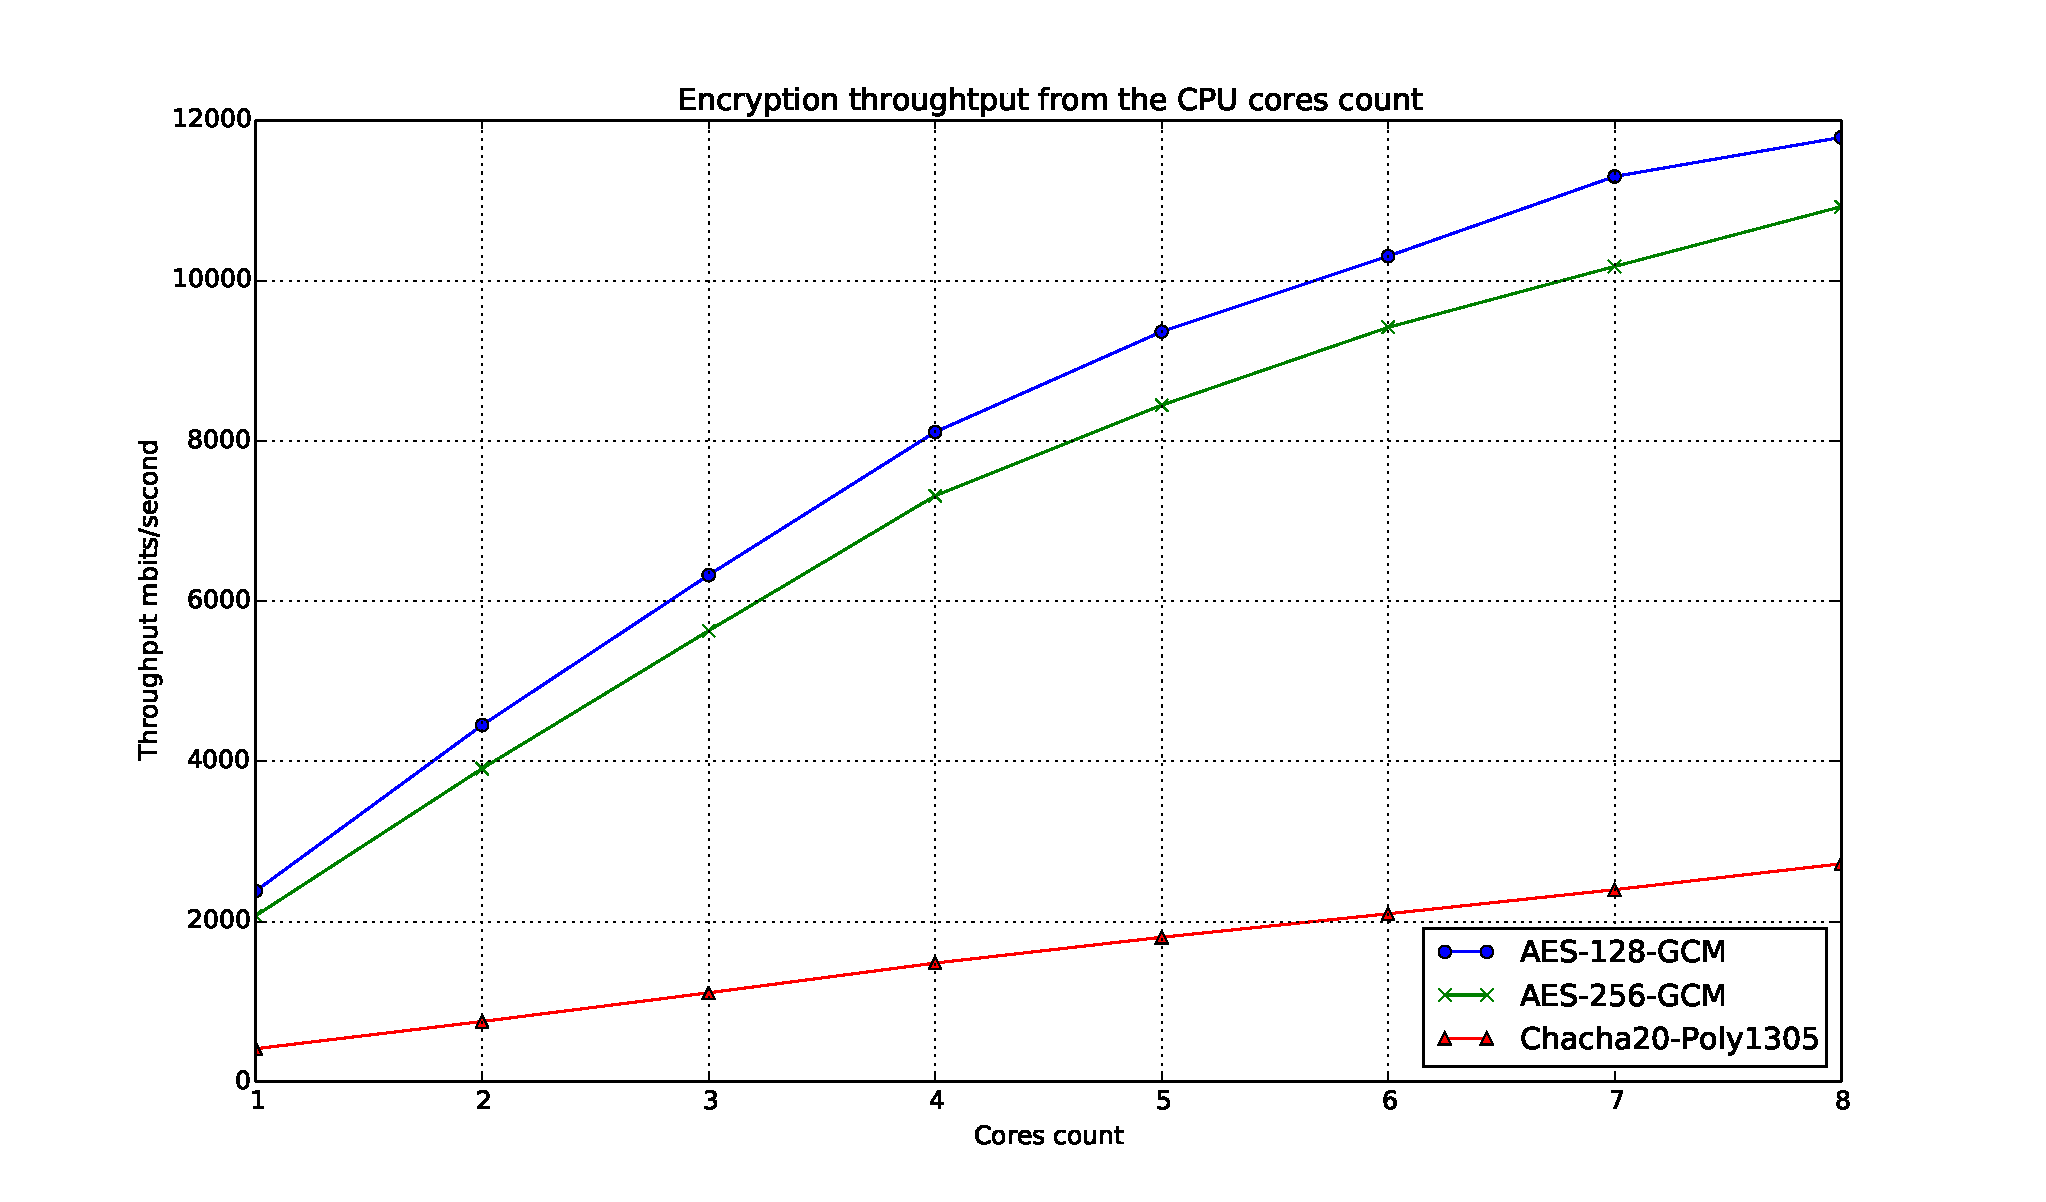
\includegraphics[height=0.6\textheight]{perf-e7.pdf}
\caption{XeonE7, 2.1 GHz, 8 CPU cores}
\end{figure}
\end{frame}

\begin{frame}
\frametitle{How expensive is encryption nowadays}
\framesubtitle{Hardware performance}
2012: Sandy Bridge (AVX, AES-NI):
\begin{figure}[H]
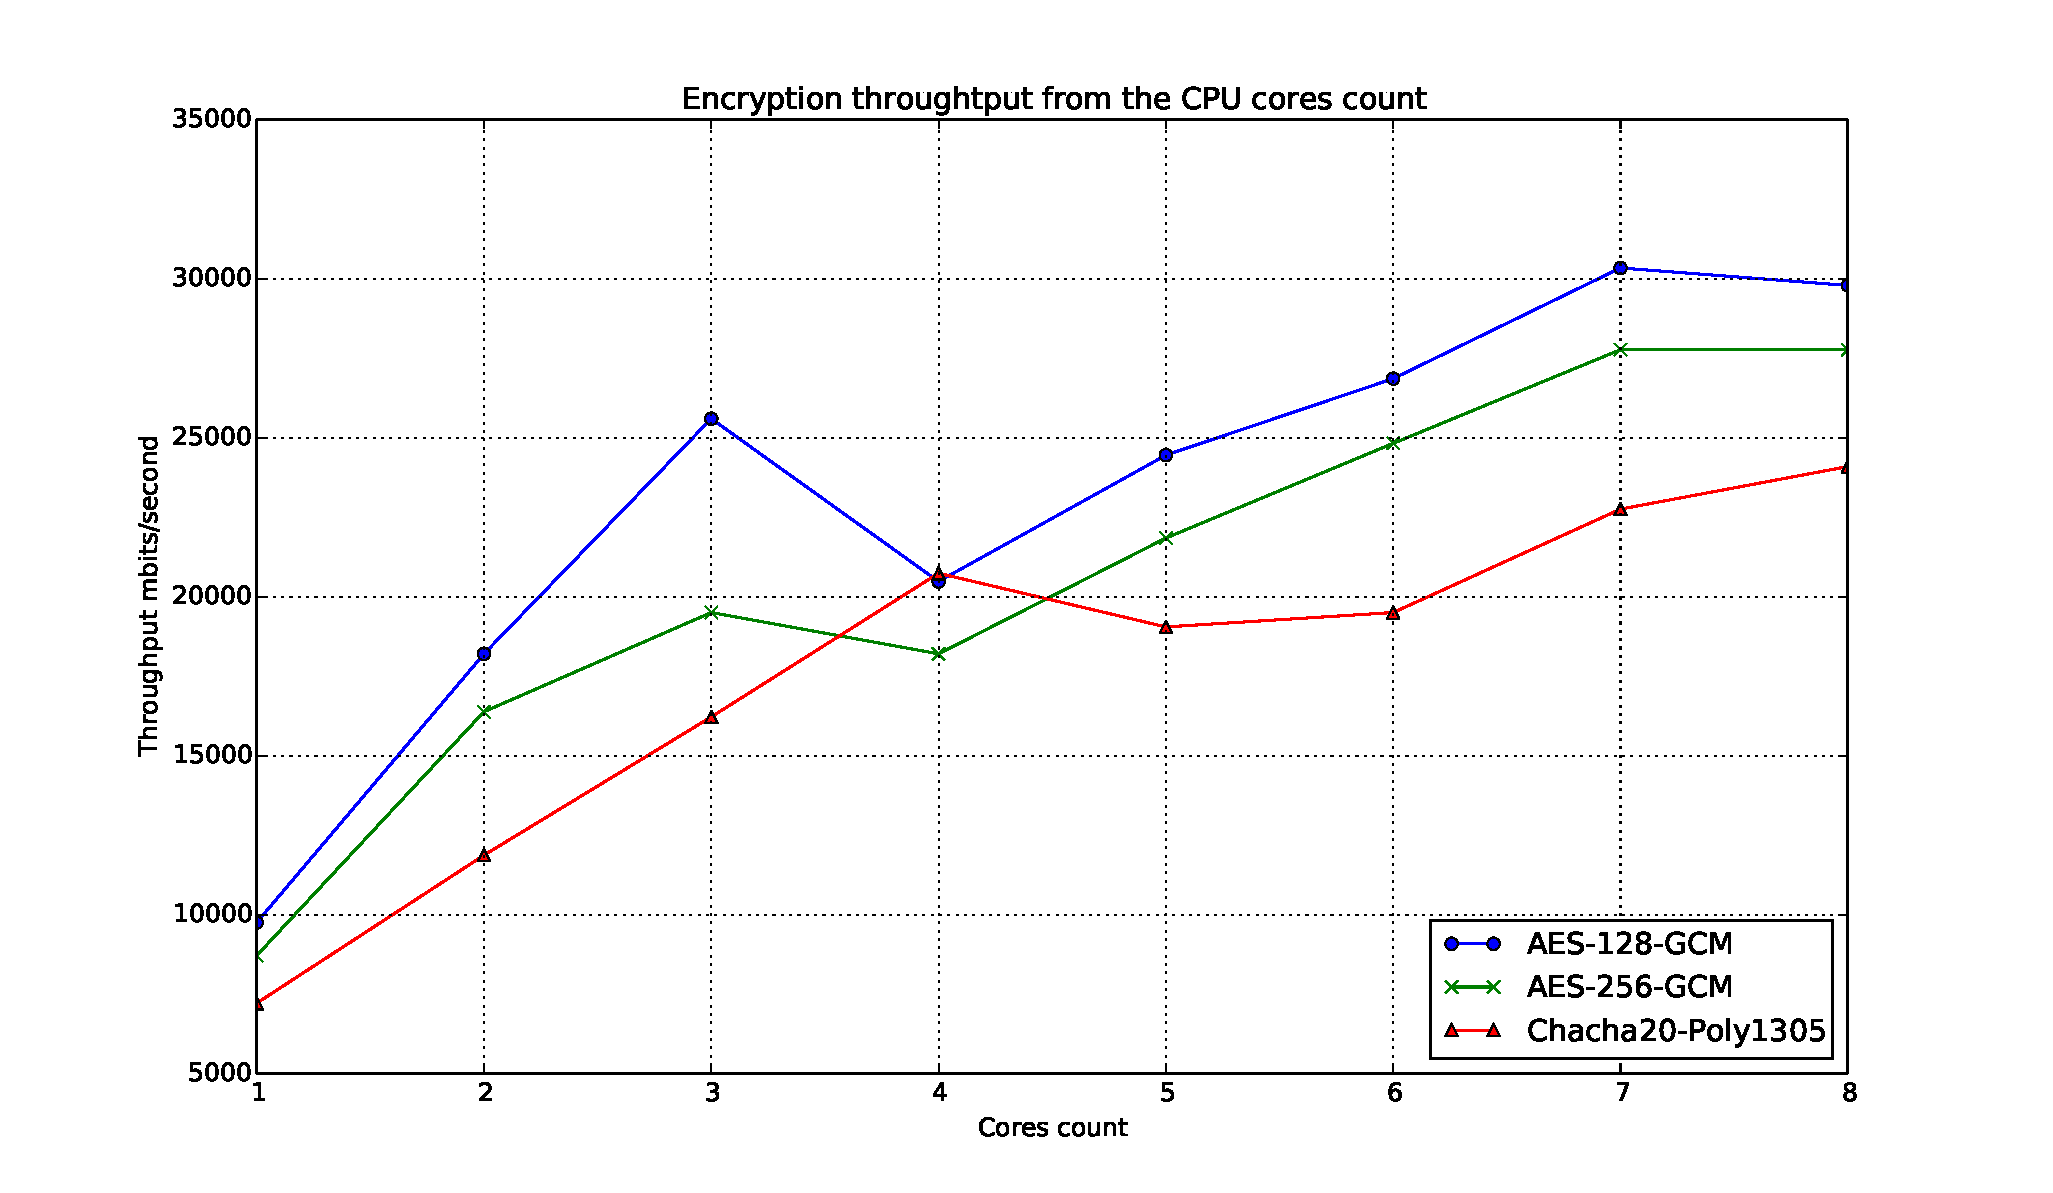
\includegraphics[height=0.6\textheight]{perf-e3.pdf}
\caption{Xeon E3, 3.4 GHz, 8 CPU cores}
\end{figure}
\end{frame}

\begin{frame}
\frametitle{How expensive is encryption nowadays}
\framesubtitle{Hardware performance}
2013: Haswell (AVX2, AES-NI):
\begin{figure}[H]
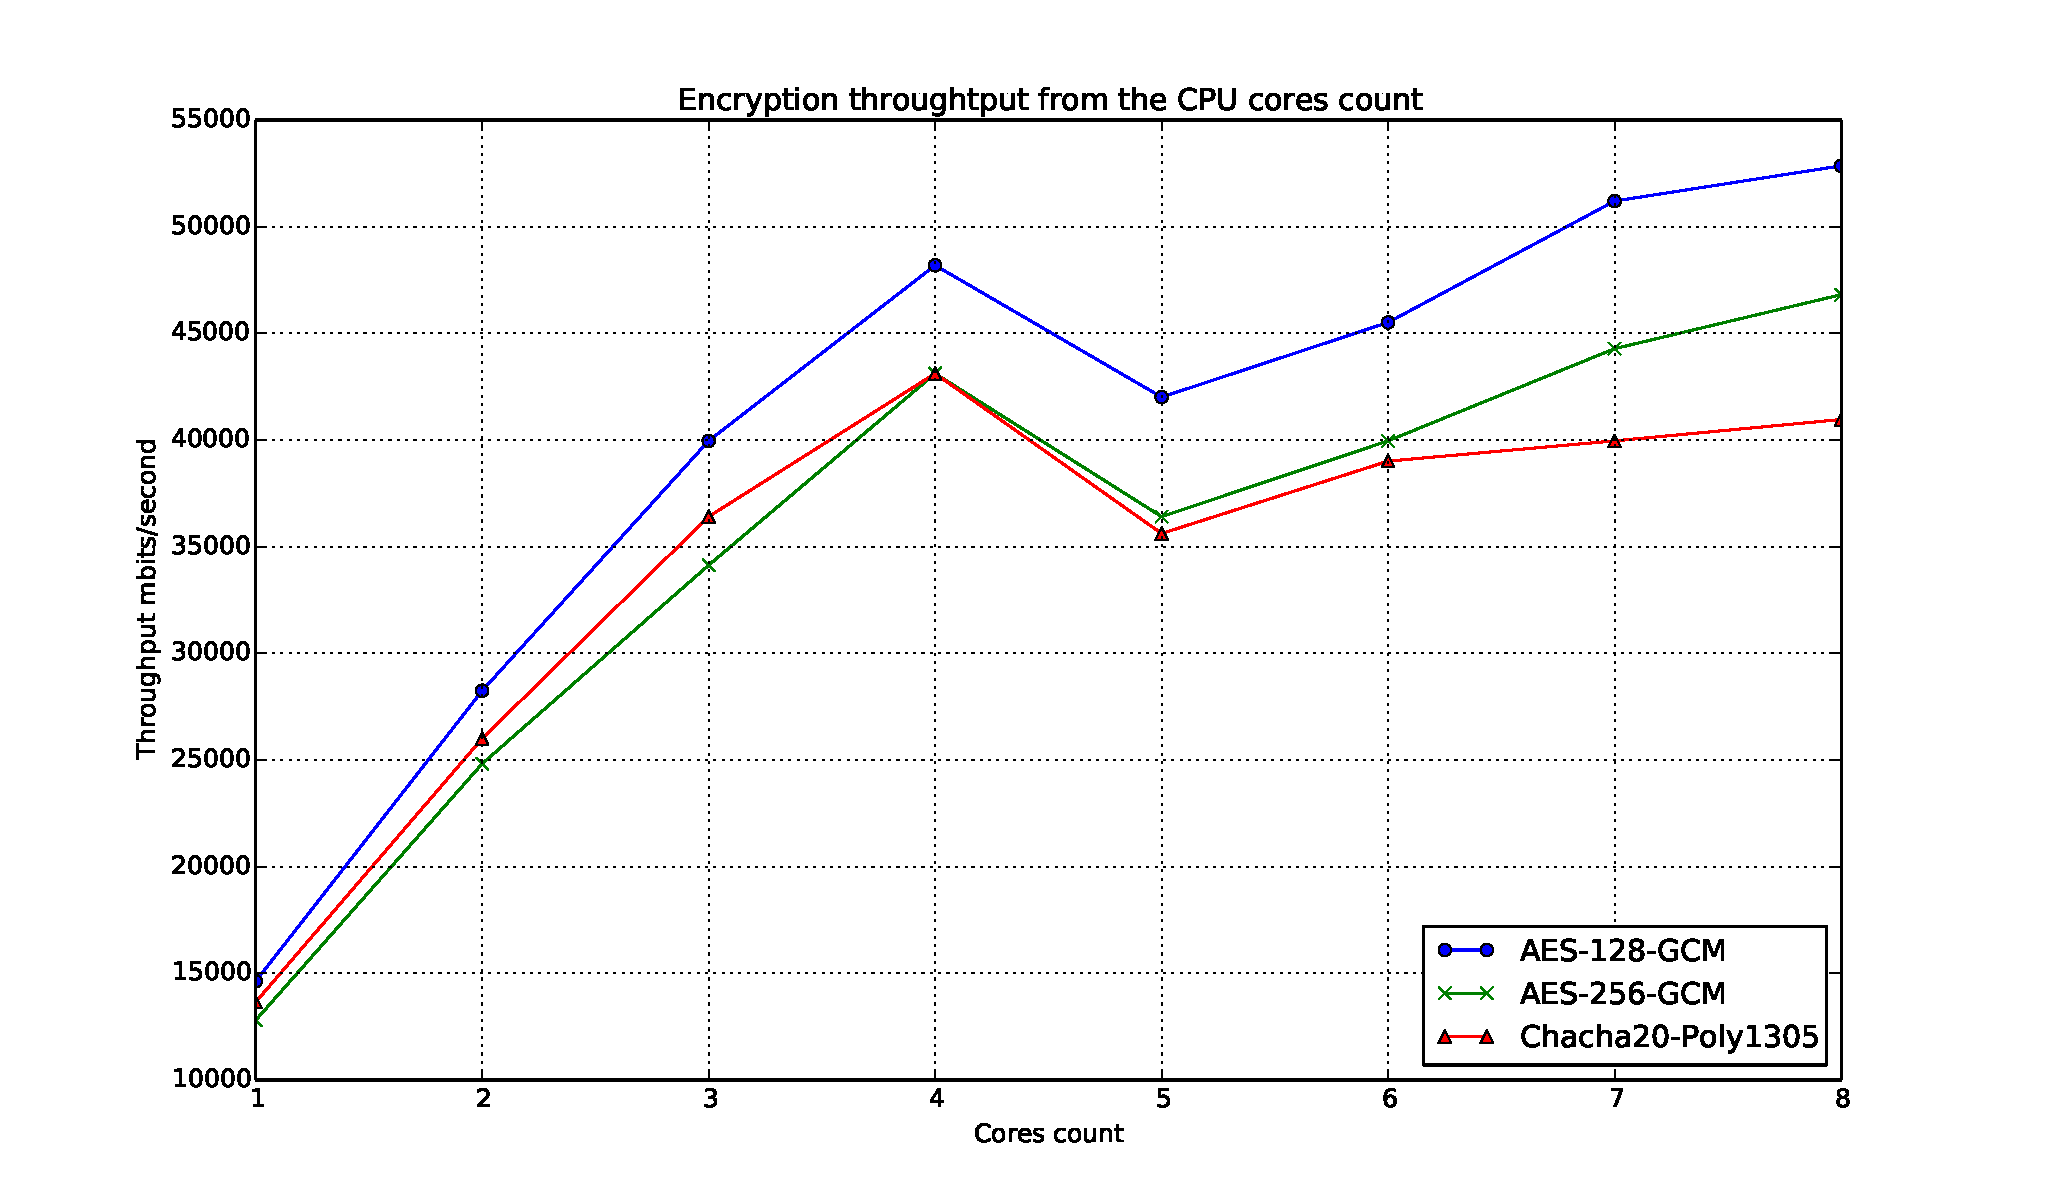
\includegraphics[height=0.6\textheight]{perf-i7.pdf}
\caption{Core-i7 4770, 3.5 GHz, 8 CPU cores}
\end{figure}
\end{frame}

\begin{frame}
\frametitle{How expensive is encryption nowadays}
\framesubtitle{Hardware performance}
Pre-historic ages: Core2 quad (SSE3):
\begin{figure}[H]
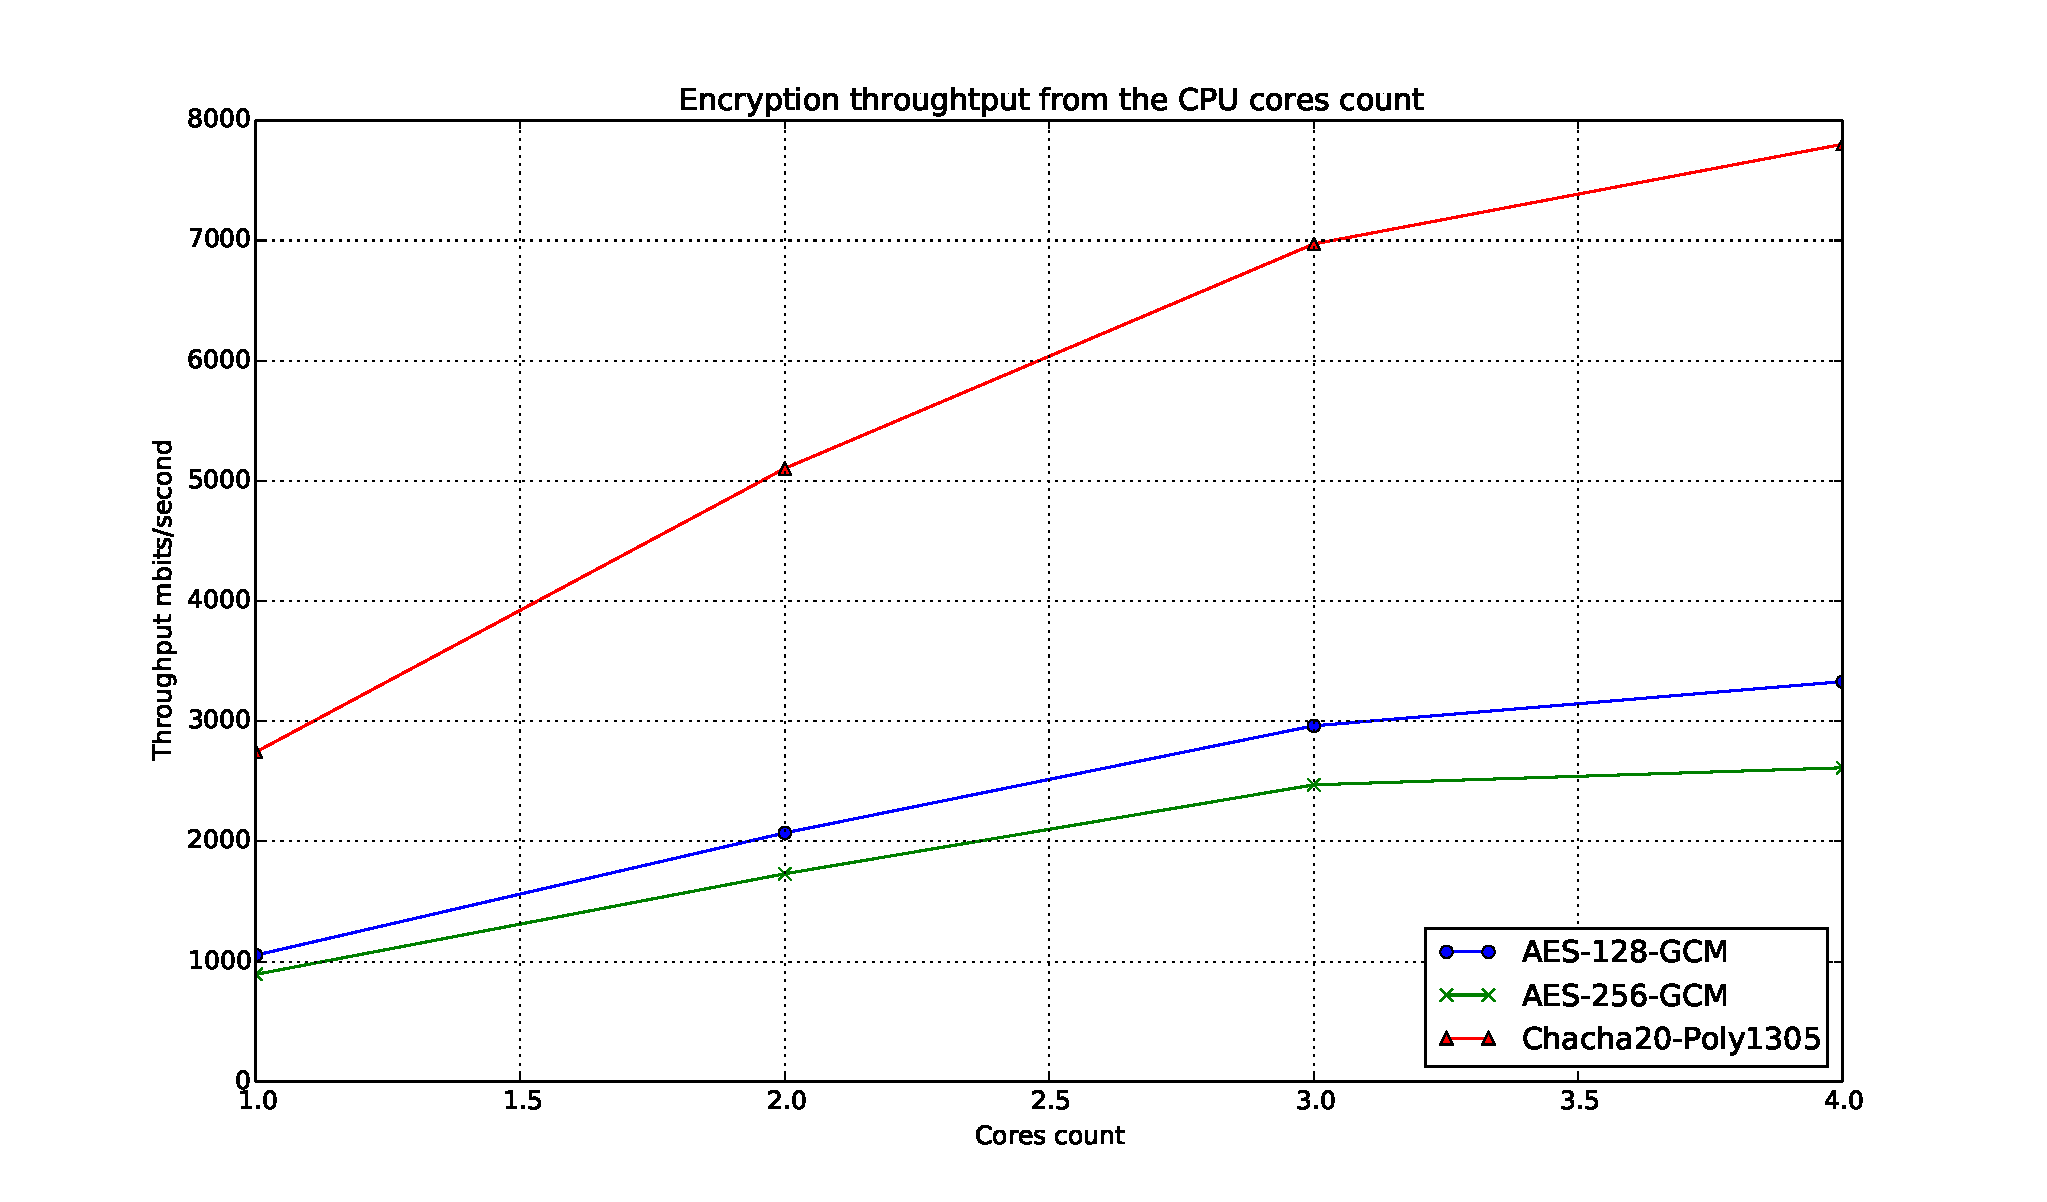
\includegraphics[height=0.6\textheight]{perf-c2.pdf}
\caption{Core2-quad, 1.5 GHz, 4 CPU cores}
\end{figure}
\end{frame}

\begin{frame}
\frametitle{How expensive is encryption nowadays}
\framesubtitle{Algorithm performance} 
3DES:
	\begin{itemize}
	\item very small block size (64 bits)
	\item need to rekey after 32 GB data
	\item need some additional MAC algorithm
	\item terribly slow
	\end{itemize}
\end{frame}

\begin{frame}[fragile]
\frametitle{How expensive is encryption nowadays}
Protocols performance:
\begin{figure}[H]
\centering
\begin{sequencediagram}
\newthread{c}{Client}
\newinst[3]{s}{Server}
\bloodymess{c}{}{s}{R}{ClientHello}{}
\begin{sdblock}[green!20]{Certificates}{}
\bloodymess{s}{CertificatesChain}{c}{L}{}{}
\end{sdblock}
\bloodymess{c}{ClientKeyExchange}{s}{R}{CertificateVerify}{}
\bloodymess{s}{}{c}{L}{ChangeCipher}{}
\end{sequencediagram}
\caption{TLS connection establishment}
\end{figure}
\end{frame}

\begin{frame}[fragile]
\frametitle{How expensive is encryption nowadays}
TLS latency improvements:
\begin{itemize}
\item Shorter certificates chain
\item Elliptic curve certificates and key exchange (ECDHE)
\item 
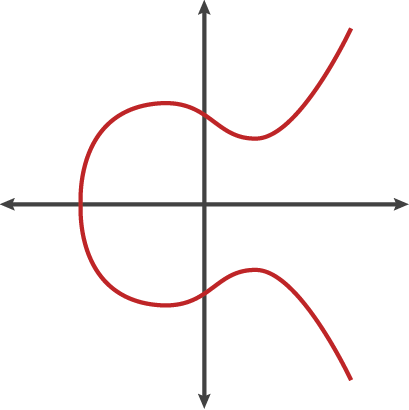
\includegraphics[height=0.2\textheight]{ec.png}
\end{itemize}
\end{frame}

\begin{frame}
\frametitle{Performance: summary}
\begin{itemize}
	\item<1-> Why use plaintext protocols?
	\item<2-> Why use old algorithms?
	\item<3-> Fast crypto in kernel (FreeBSD-HEAD by jmg@)
	\item<4-> But initial latency for secure connections is still high.
\end{itemize}
\end{frame}

\end{document}